\[
    \left|
    \begin{gathered}
        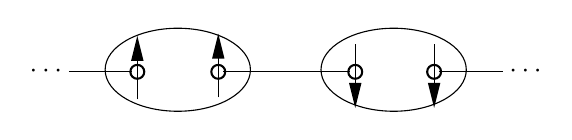
\begin{tikzpicture}[x=0.75pt,y=0.75pt,yscale=-1,xscale=1]
            %uncomment if require: \path (0,300); %set diagram left start at 0, and has height of 300
            
            %Straight Lines [id:da4083072976683597] 
            \draw    (128.5,145) -- (159.15,145) ;
            \draw [shift={(161.5,145)}, rotate = 0] [color={rgb, 255:red, 0; green, 0; blue, 0 }  ][line width=0.75]      (0, 0) circle [x radius= 3.35, y radius= 3.35]   ;
            %Straight Lines [id:da6245903945041391] 
            \draw    (202.85,145) -- (233.5,145) ;
            \draw [shift={(200.5,145)}, rotate = 0] [color={rgb, 255:red, 0; green, 0; blue, 0 }  ][line width=0.75]      (0, 0) circle [x radius= 3.35, y radius= 3.35]   ;
            %Shape: Ellipse [id:dp26280268474606805] 
            \draw   (146,144) .. controls (146,132.95) and (161.67,124) .. (181,124) .. controls (200.33,124) and (216,132.95) .. (216,144) .. controls (216,155.05) and (200.33,164) .. (181,164) .. controls (161.67,164) and (146,155.05) .. (146,144) -- cycle ;
            %Straight Lines [id:da6652029642623027] 
            \draw    (233.5,145) -- (264.15,145) ;
            \draw [shift={(266.5,145)}, rotate = 0] [color={rgb, 255:red, 0; green, 0; blue, 0 }  ][line width=0.75]      (0, 0) circle [x radius= 3.35, y radius= 3.35]   ;
            %Straight Lines [id:da24190764323274072] 
            \draw    (306.85,145) -- (337.5,145) ;
            \draw [shift={(304.5,145)}, rotate = 0] [color={rgb, 255:red, 0; green, 0; blue, 0 }  ][line width=0.75]      (0, 0) circle [x radius= 3.35, y radius= 3.35]   ;
            %Shape: Ellipse [id:dp39498555042265426] 
            \draw   (250,144) .. controls (250,132.95) and (265.67,124) .. (285,124) .. controls (304.33,124) and (320,132.95) .. (320,144) .. controls (320,155.05) and (304.33,164) .. (285,164) .. controls (265.67,164) and (250,155.05) .. (250,144) -- cycle ;
            %Straight Lines [id:da19523581731330353] 
            \draw    (200.5,157.33) -- (200.5,128.67) ;
            \draw [shift={(200.5,126.67)}, rotate = 450] [fill={rgb, 255:red, 0; green, 0; blue, 0 }  ][line width=0.08]  [draw opacity=0] (12,-3) -- (0,0) -- (12,3) -- cycle    ;
            %Straight Lines [id:da0670010109307011] 
            \draw    (266.5,131.67) -- (266.5,160.33) ;
            \draw [shift={(266.5,162.33)}, rotate = 270] [fill={rgb, 255:red, 0; green, 0; blue, 0 }  ][line width=0.08]  [draw opacity=0] (12,-3) -- (0,0) -- (12,3) -- cycle    ;
            %Straight Lines [id:da5441943573714076] 
            \draw    (161.5,158.33) -- (161.5,129.67) ;
            \draw [shift={(161.5,127.67)}, rotate = 450] [fill={rgb, 255:red, 0; green, 0; blue, 0 }  ][line width=0.08]  [draw opacity=0] (12,-3) -- (0,0) -- (12,3) -- cycle    ;
            %Straight Lines [id:da2924742628965573] 
            \draw    (304.5,131.67) -- (304.5,160.33) ;
            \draw [shift={(304.5,162.33)}, rotate = 270] [fill={rgb, 255:red, 0; green, 0; blue, 0 }  ][line width=0.08]  [draw opacity=0] (12,-3) -- (0,0) -- (12,3) -- cycle    ;
            
            % Text Node
            \draw (126.5,145) node [anchor=east] [inner sep=0.75pt]    {$\cdots $};
            % Text Node
            \draw (339.5,145) node [anchor=west] [inner sep=0.75pt]    {$\cdots $};
            \end{tikzpicture} 
    \end{gathered} %
    \right\rangle
    + \left|
    \begin{gathered}
        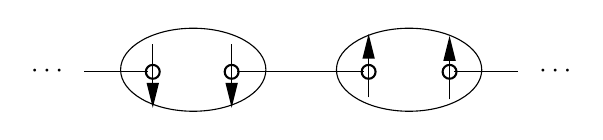
\begin{tikzpicture}[x=0.75pt,y=0.75pt,yscale=-1,xscale=1]
            %uncomment if require: \path (0,300); %set diagram left start at 0, and has height of 300
            
            %Straight Lines [id:da017781333983049485] 
            \draw    (357.5,165) -- (326.85,165) ;
            \draw [shift={(324.5,165)}, rotate = 180] [color={rgb, 255:red, 0; green, 0; blue, 0 }  ][line width=0.75]      (0, 0) circle [x radius= 3.35, y radius= 3.35]   ;
            %Straight Lines [id:da8236611936981324] 
            \draw    (283.15,165) -- (252.5,165) ;
            \draw [shift={(285.5,165)}, rotate = 180] [color={rgb, 255:red, 0; green, 0; blue, 0 }  ][line width=0.75]      (0, 0) circle [x radius= 3.35, y radius= 3.35]   ;
            %Shape: Ellipse [id:dp6056385400541942] 
            \draw   (340,164) .. controls (340,152.95) and (324.33,144) .. (305,144) .. controls (285.67,144) and (270,152.95) .. (270,164) .. controls (270,175.05) and (285.67,184) .. (305,184) .. controls (324.33,184) and (340,175.05) .. (340,164) -- cycle ;
            %Straight Lines [id:da5068839528018145] 
            \draw    (252.5,165) -- (221.85,165) ;
            \draw [shift={(219.5,165)}, rotate = 180] [color={rgb, 255:red, 0; green, 0; blue, 0 }  ][line width=0.75]      (0, 0) circle [x radius= 3.35, y radius= 3.35]   ;
            %Straight Lines [id:da23040796825816323] 
            \draw    (179.15,165) -- (148.5,165) ;
            \draw [shift={(181.5,165)}, rotate = 180] [color={rgb, 255:red, 0; green, 0; blue, 0 }  ][line width=0.75]      (0, 0) circle [x radius= 3.35, y radius= 3.35]   ;
            %Shape: Ellipse [id:dp9527924399977281] 
            \draw   (236,164) .. controls (236,152.95) and (220.33,144) .. (201,144) .. controls (181.67,144) and (166,152.95) .. (166,164) .. controls (166,175.05) and (181.67,184) .. (201,184) .. controls (220.33,184) and (236,175.05) .. (236,164) -- cycle ;
            %Straight Lines [id:da1189241220265258] 
            \draw    (285.5,177.33) -- (285.5,148.67) ;
            \draw [shift={(285.5,146.67)}, rotate = 450] [fill={rgb, 255:red, 0; green, 0; blue, 0 }  ][line width=0.08]  [draw opacity=0] (12,-3) -- (0,0) -- (12,3) -- cycle    ;
            %Straight Lines [id:da7736984694103599] 
            \draw    (219.5,151.67) -- (219.5,180.33) ;
            \draw [shift={(219.5,182.33)}, rotate = 270] [fill={rgb, 255:red, 0; green, 0; blue, 0 }  ][line width=0.08]  [draw opacity=0] (12,-3) -- (0,0) -- (12,3) -- cycle    ;
            %Straight Lines [id:da7040925530597031] 
            \draw    (324.5,178.33) -- (324.5,149.67) ;
            \draw [shift={(324.5,147.67)}, rotate = 450] [fill={rgb, 255:red, 0; green, 0; blue, 0 }  ][line width=0.08]  [draw opacity=0] (12,-3) -- (0,0) -- (12,3) -- cycle    ;
            %Straight Lines [id:da8290985403901272] 
            \draw    (181.5,151.67) -- (181.5,180.33) ;
            \draw [shift={(181.5,182.33)}, rotate = 270] [fill={rgb, 255:red, 0; green, 0; blue, 0 }  ][line width=0.08]  [draw opacity=0] (12,-3) -- (0,0) -- (12,3) -- cycle    ;
            
            % Text Node
            \draw (384.5,165) node [anchor=west] [inner sep=0.75pt]  [xscale=-1]  {$\cdots $};
            % Text Node
            \draw (121.5,165) node [anchor=east] [inner sep=0.75pt]  [xscale=-1]  {$\cdots $};
            \end{tikzpicture}
    \end{gathered}
    \right\rangle
\]